
\section{Speed: Distance and Time}
\label{sec:speed}

We have modelled a trackway as a row of dots. To turn the dots into a number, we need to say precisely what speed is.

\subsection{The basic relationship}

Before Galileo, people described motion as simply ``fast'' or ``slow.'' Galileo is credited with being the first to \emph{measure} speed, by comparing the distance covered with the time taken. His definition is still ours.

\begin{definition}{Speed}{speed}
The \textbf{speed} of an object is the distance it covers per unit of time:
\[
\text{speed} = \frac{\text{distance}}{\text{time}}, \qquad v = \frac{d}{t}.
\]
The SI unit is the metre per second, \si{\metre\per\second}. Rearranged, the same relationship reads $d = v t$ (distance is speed times time) and $t = d/v$ (time is distance divided by speed).
\end{definition}

Take the definition apart. For a fixed time, a larger distance means a larger speed: an object that goes \SI{500}{\metre} in \SI{10}{\second} is faster than one that goes \SI{5}{\metre} in \SI{10}{\second}. For a fixed distance, a \emph{smaller} time means a larger speed, because dividing by a smaller number gives a bigger result: an object that covers \SI{10}{\metre} in \SI{0.02}{\second} is a hundred times faster than one that covers \SI{10}{\metre} in \SI{2}{\second}. Both halves of the fraction pull in the directions common sense expects.

\begin{twoviews}{speed, distance, and time}
\elem If you travel at a steady \SI{30}{\kilo\metre\per\hour} for \SI{2}{\hour}, you cover \SI{60}{\kilo\metre}: each hour contributes \SI{30}{\kilo\metre}, and there are two of them. In general, distance is speed times time, $d = vt$, and this is just the definition $v = d/t$ multiplied through by $t$. On a graph of speed against time, a steady speed is a horizontal line, and $vt$ is the area of the rectangle beneath it: height $v$, width $t$. If the speed changes in steps (\SI{30}{\kilo\metre\per\hour} for one hour, then \SI{50}{\kilo\metre\per\hour} for the next), add the rectangles: \SI{80}{\kilo\metre}.

\calc Let $x(t)$ be the object's position along its line of motion, measured from some chosen origin. Its speed at the instant $t$ is the rate at which $x$ changes, the derivative
\[
v(t) = \deriv{x}{t}.
\]
Distance is recovered by integrating the speed over the time interval concerned:
\[
d = \int_{t_1}^{t_2} v(t)\,\dd t,
\]
the area under the speed--time graph between $t_1$ and $t_2$. When $v$ is a constant, the integral is $v\,(t_2 - t_1)$, the rectangle of the elementary route. When $v$ changes in steps, the integral is the sum of rectangles. When $v$ changes smoothly, the integral is still the area, and the elementary route can only approximate it by thin rectangles; the integral gives it exactly. The definition $v = d/t$ is the special case of the derivative in which the rate happens to be constant.
\end{twoviews}

\begin{example}{Walking speed from stride data}{walking}
You walk at a steady pace, taking one stride every \SI{1.12}{\second}, and your stride length is \SI{1.46}{\metre}. How fast are you walking, in metres per second?

\elem Draw the dot diagram first: dots \SI{1.46}{\metre} apart, $\tau = \SI{1.12}{\second}$. One gap is one stride, so
\[
v = \frac{d}{t} = \frac{\SI{1.46}{\metre}}{\SI{1.12}{\second}} = \SI{1.30}{\metre\per\second}.
\]
The units come out as metres divided by seconds, which is what a speed should be. As a sanity check, \SI{1.30}{\metre\per\second} is about \SI{4.7}{\kilo\metre\per\hour}, or a little under \SI{3}{\mile\per\hour}; it would take about $\SI{1000}{\metre}/\SI{1.30}{\metre\per\second} = \SI{770}{\second} \approx \SI{13}{\minute}$ to walk a kilometre. That is an ordinary walking pace, so the answer is believable.

\calc The position of your right foot is a function of time that jumps forward by \SI{1.46}{\metre} once every \SI{1.12}{\second}; your body's position $x(t)$ is smoother, but it advances by the same \SI{1.46}{\metre} every \SI{1.12}{\second}. Over any whole number $n$ of strides,
\[
\int_{0}^{n\tau} v\,\dd t = x(n\tau) - x(0) = n \times \SI{1.46}{\metre},
\]
so the mean value of $v$ over that time is $(n \times 1.46)/(n \times 1.12) = \SI{1.30}{\metre\per\second}$, whatever $n$ is. Within a single stride your speed rises and falls slightly as you push off and land, so $\dd x/\dd t$ wobbles around \SI{1.30}{\metre\per\second}; the dot diagram averages over that wobble, which is exactly what we want.\qed
\end{example}

We did not strictly need the dot diagram to do the arithmetic, but drawing it first is a habit worth forming. It makes you write down what you know ($\tau$, the spacing) and notice what you do not. Had the problem given only the stride length, you could draw the dots but not find the speed: you would know how far apart the dots are but not how much time separates them. That is precisely Webb's situation with the hunter. He could measure the stride length but not the time between strides, and Section~\ref{sec:stridemodel} is about how he filled the gap.

\subsection{Solving for time or distance}

The relationship $v = d/t$ contains three quantities, and any two determine the third.

\begin{example}{Paint drops from a wheel}{wheel}
A car travels along a straight road at a steady \SI{22}{\metre\per\second}. A blob of wet paint on one tyre leaves a mark on the road once per revolution, and the wheel turns once every \SI{0.088}{\second}. (a) How far apart are the marks? (b) What does that distance represent physically, and what is the wheel's diameter?

\elem (a) Distance is speed times time:
\[
d = vt = \SI{22}{\metre\per\second} \times \SI{0.088}{\second} = \SI{1.94}{\metre}.
\]
Check the units: (\si{\metre\per\second})(\si{\second}) $=$ \si{\metre}, as required. (b) The car moves \SI{1.94}{\metre} during one turn of the wheel, and a rolling wheel that does not skid advances by exactly its own circumference per turn. So \SI{1.94}{\metre} is the tyre's circumference, and the diameter is $1.94/\pi = \SI{0.62}{\metre}$, a reasonable size for a car tyre. The paint marks are a dot diagram with $\tau = \SI{0.088}{\second}$, drawn by the car itself.

\calc With $v$ constant, $\int_{0}^{0.088} 22\,\dd t = 22 \times 0.088 = \SI{1.94}{\metre}$; nothing more is needed. The calculus reading of part (b) is that the wheel's angle $\theta(t)$ and the car's position $x(t)$ are locked together by $x = r\theta$ for a wheel of radius $r$ that rolls without slipping, so $\dd x/\dd t = r\,\dd\theta/\dd t$; one full turn ($\Delta\theta = 2\pi$) advances the car by $2\pi r$, the circumference.\qed
\end{example}

\begin{example}{Finding the time between strides}{stridetime}
A runner moves at \SI{3.0}{\metre\per\second} with a stride length of \SI{2.20}{\metre}. How much time passes between successive strides?

\solution Solve $v = d/t$ for the time: $t = d/v$. Then
\[
t = \frac{\SI{2.20}{\metre}}{\SI{3.0}{\metre\per\second}} = \SI{0.73}{\second}.
\]
Units: metres divided by metres-per-second leaves seconds, as it should. About three quarters of a second per stride, or roughly \num{80} strides a minute, is typical of an easy distance-running pace. \calctag\ If the speed were not constant the time to cover \SI{2.20}{\metre} would be the $t$ for which $\int_0^t v\,\dd t' = 2.20$, which for constant $v$ reduces to $vt = 2.20$.\qed
\end{example}

\subsection{Comparing diagrams by ratios}

Sometimes you are given no numbers at all, only how two situations compare. The definition of speed handles that too, because it says how $v$ \emph{scales} when $d$ or $t$ is scaled.

\begin{example}{Two diagrams, two intervals}{scaling}
Two dot diagrams are made for objects A and B. The dots in diagram A are three times as far apart as those in diagram B, but diagram A was recorded with twice the time between dots. (a) Which object is faster, and by what factor? (b) If B moves at \SI{8.0}{\metre\per\second}, how fast does A move?

\elem Work from B to A one change at a time. Tripling the distance between dots, with the time held fixed, would triple the speed. Doubling the time between dots, with the distance held fixed, would halve the speed. Both changes together multiply the speed by $3 \times \tfrac12 = \tfrac32$. So A is faster, by a factor of \num{1.5}, and $v_A = 1.5 \times \SI{8.0}{\metre\per\second} = \SI{12}{\metre\per\second}$. If you prefer concrete numbers, invent some: let B have dots \SI{1}{\metre} apart every \SI{1}{\second} (speed \SI{1}{\metre\per\second}); then A has dots \SI{3}{\metre} apart every \SI{2}{\second} (speed \SI{1.5}{\metre\per\second}). The made-up numbers cancel out of the ratio.

\calc Write $v_A = d_A/\tau_A$ and $v_B = d_B/\tau_B$. Then
\[
\frac{v_A}{v_B} = \frac{d_A}{d_B}\cdot\frac{\tau_B}{\tau_A} = 3 \times \frac12 = \frac32,
\]
which is the same bookkeeping written as one fraction. A useful way to see it: $v$ is proportional to $d$ and inversely proportional to $\tau$, so $\ln v = \ln d - \ln \tau + \text{const}$, and small fractional changes add: a $+200\%$ change in $d$ and a $+100\%$ change in $\tau$ combine as a factor $3/2$. Physicists use this ``multiply the factors'' habit constantly, and it is worth practising until it is automatic.\qed
\end{example}

\begin{checkbox}
A dot diagram has dots \SI{4}{\centi\metre} apart with \SI{8}{\second} between dots. Find the speed in \si{\metre\per\second} and in \si{\centi\metre\per\second}, and name an animal that moves at about that speed.
\end{checkbox}

\subsection{Units and conversions}

Any distance unit divided by any time unit is a legitimate speed unit. Road signs use kilometres per hour or miles per hour; athletics uses metres per second; sailors use knots (nautical miles per hour); geologists measure the drift of continents in centimetres per year. Physics uses \si{\metre\per\second} by default, and you will need to move between units fluently. Table~\ref{tab:speeds} gives some landmarks.

\begin{table}[htb]
\centering
\caption{Some speeds in three units. The conversions use $\SI{1}{\hour} = \SI{3600}{\second}$ and $\SI{1}{\mile} = \SI{1609.344}{\metre}$, so $\SI{1}{\metre\per\second} = \SI{3.6}{\kilo\metre\per\hour} = \SI{2.237}{\mile\per\hour}$. The first six rows are adapted from Hewitt's Table~3.1.}
\label{tab:speeds}
\renewcommand{\arraystretch}{1.2}
\begin{tabular}{lccc}
\toprule
 & \si{\metre\per\second} & \si{\kilo\metre\per\hour} & \si{\mile\per\hour} \\
\midrule
brisk walk & 1.5 & 5.4 & 3.4 \\
 & 5 & 18 & 11 \\
 & 10 & 36 & 22 \\
 & 20 & 72 & 45 \\
 & 30 & 108 & 67 \\
 & 40 & 144 & 89 \\
 & 50 & 180 & 112 \\
sound in air (\SI{20}{\celsius}) & 343 & 1235 & 767 \\
\bottomrule
\end{tabular}
\end{table}

The safe way to convert is to multiply by fractions equal to one. Since $\SI{1}{\kilo\metre} = \SI{1000}{\metre}$, the fraction $(\SI{1000}{\metre})/(\SI{1}{\kilo\metre})$ equals one and can be inserted anywhere without changing a value; it only changes the units in which the value is written. Units cancel like algebraic symbols.

\begin{example}{Converting a sprinter's average speed}{convert}
Usain Bolt's world record for \SI{100}{\metre}, set in Berlin in 2009, is \SI{9.58}{\second}. Find his average speed in \si{\metre\per\second}, \si{\kilo\metre\per\hour}, and \si{\mile\per\hour}.

\solution In SI units,
\[
v = \frac{\SI{100}{\metre}}{\SI{9.58}{\second}} = \SI{10.44}{\metre\per\second}.
\]
Convert to kilometres per hour by multiplying by two fractions equal to one:
\[
\SI{10.44}{\metre\per\second} \times \frac{\SI{1}{\kilo\metre}}{\SI{1000}{\metre}} \times \frac{\SI{3600}{\second}}{\SI{1}{\hour}} = \SI{37.6}{\kilo\metre\per\hour}.
\]
Metres cancel against metres and seconds against seconds, leaving \si{\kilo\metre\per\hour}. (The shortcut ``multiply by \num{3.6}'' is these two fractions combined.) Then, using $\SI{1}{\mile} = \SI{1.609}{\kilo\metre}$,
\[
\SI{37.6}{\kilo\metre\per\hour} \times \frac{\SI{1}{\mile}}{\SI{1.609}{\kilo\metre}} = \SI{23.4}{\mile\per\hour}.
\]
Sanity check against Table~\ref{tab:speeds}: \SI{10}{\metre\per\second} is \SI{36}{\kilo\metre\per\hour} and \SI{22}{\mile\per\hour}, and Bolt's numbers are all slightly above those. A fit cyclist on the flat can hold \SI{37}{\kilo\metre\per\hour}; a sprinter matches it for ten seconds.\qed
\end{example}

\begin{modelnote}[Let the units do the checking]
Carrying units through every step costs a few seconds and catches a large fraction of all mistakes. If you divide when you should have multiplied, the units will come out as \si{\second\per\metre} instead of \si{\metre\per\second} and you will notice. If a formula you half-remember gives an answer in \si{\metre\squared}, it is not a speed, whatever the number says. Treat a unit mismatch as a certain sign of error, and treat matching units as necessary but not sufficient: the right units with the wrong number is still wrong.
\end{modelnote}

\subsection{Average speed and instantaneous speed}
\label{sec:instant}

The speedometer of a car reads \SI{50}{\kilo\metre\per\hour} at one moment, \num{0} at a red light a minute later, and \num{30} in traffic after that. The reading at any one moment is the car's \textbf{instantaneous speed}. It says: \emph{if} the car kept going exactly like this for an hour, it would cover \SI{50}{\kilo\metre}. It does not say the car will do so, only what it is doing now.

On a long trip the driver cares about something different: how far in how long. That is the \textbf{average speed}, total distance divided by total time. If the trip covers \SI{320}{\kilo\metre} in \SI{4}{\hour}, the average speed is \SI{80}{\kilo\metre\per\hour}, and no information about the traffic light survives in that number.

\begin{definition}{Average and instantaneous speed}{avginst}
The \textbf{average speed} over a time interval is
\[
\bar v = \frac{\text{total distance covered}}{\text{time interval}}.
\]
The \textbf{instantaneous speed} at an instant is the average speed over a very short interval containing that instant, so short that shortening it further does not change the answer. \elemtag\ It is what a speedometer reads. \calctag\ It is the derivative $v = \dd x/\dd t$, the limit of $\Delta x/\Delta t$ as $\Delta t \to 0$. When this book says ``speed'' without qualification it means the instantaneous speed.
\end{definition}

Unless the speed is steady, the two are different, and the difference matters. A police officer who clocks you at \SI{140}{\kilo\metre\per\hour} writes the instantaneous speed on the ticket; that your \emph{average} over the whole journey was a lawful \SI{80}{\kilo\metre\per\hour} is no defence.

\begin{twoviews}{instantaneous speed}
\elem Suppose you know an object's position at many closely spaced times. To estimate its speed at one particular instant, take the positions a little before and a little after, subtract, and divide by the time between them. Then shrink the interval and repeat. The ratios settle down to a definite number, and that number is the instantaneous speed. There is nothing more to it than average speed over an interval you keep making shorter. The only limit on the method is practical: real position data have a finite resolution, and below some interval the ratio starts to be dominated by measurement noise.

\calc The settling-down of the ratios is what a \emph{limit} is, and the limit of $\Delta x/\Delta t$ as $\Delta t \to 0$ is the derivative:
\[
v(t) = \lim_{\Delta t \to 0}\frac{x(t + \Delta t) - x(t)}{\Delta t} = \deriv{x}{t}.
\]
When $x(t)$ is given by a formula, the rules of differentiation deliver $v(t)$ directly, with no shrinking intervals to tabulate. When $x(t)$ is known only from data, the elementary procedure \emph{is} the numerical evaluation of the derivative. The average speed over an interval is, correspondingly, the mean value of $v$ over the interval:
\[
\bar v = \frac{1}{t_2 - t_1}\int_{t_1}^{t_2} v(t)\,\dd t = \frac{x(t_2) - x(t_1)}{t_2 - t_1}
\]
(for motion that does not reverse), which is the elementary definition again.
\end{twoviews}

\begin{example}{A sprinter leaving the blocks}{cubic}
For the first five seconds of a race, a sprinter's position along the track is well approximated by $x(t) = (\SI{0.10}{\metre\per\second\cubed})\,t^3$. (a) Find the sprinter's average speed over the first \SI{5.0}{\second}. (b) Find the instantaneous speed at $t = \SI{5.0}{\second}$. (c) Explain why the two differ.

\elem (a) $x(5.0) = 0.10 \times 125 = \SI{12.5}{\metre}$, so the average speed is $\SI{12.5}{\metre}/\SI{5.0}{\second} = \SI{2.5}{\metre\per\second}$. (b) Compute average speeds over shrinking intervals centred on $t = \SI{5.0}{\second}$, using $x(t) = 0.10\,t^3$:
\begin{center}
\renewcommand{\arraystretch}{1.2}
\begin{tabular}{ccccc}
\toprule
interval (s) & $x$ at start (m) & $x$ at end (m) & $\Delta x$ (m) & $\Delta x/\Delta t$ (m/s) \\
\midrule
4.0 to 6.0 & 6.400 & 21.600 & 15.200 & 7.60 \\
4.5 to 5.5 & 9.113 & 16.638 & 7.525 & 7.53 \\
4.9 to 5.1 & 11.765 & 13.265 & 1.500 & 7.50 \\
\bottomrule
\end{tabular}
\end{center}
The ratios are settling on \SI{7.5}{\metre\per\second}; a further row (\num{4.99} to \num{5.01}) would give \num{7.500}. So the instantaneous speed at \SI{5.0}{\second} is \SI{7.5}{\metre\per\second}. (c) The sprinter was slower than \SI{7.5}{\metre\per\second} for the whole five seconds except the final instant, so the average over the interval is necessarily less than the speed at its end.

\calc (b) Differentiate: $v(t) = \dd x/\dd t = 3 \times 0.10\,t^2 = 0.30\,t^2$, so $v(5.0) = 0.30 \times 25 = \SI{7.5}{\metre\per\second}$, confirming the table's limit exactly. (a) The average is the mean value of $v$:
\[
\bar v = \frac{1}{5.0}\int_0^{5.0} 0.30\,t^2\,\dd t = \frac{1}{5.0}\left[0.10\,t^3\right]_0^{5.0} = \frac{12.5}{5.0} = \SI{2.5}{\metre\per\second}.
\]
(c) Since $v(t)$ increases throughout, its mean over $[0, 5]$ is less than its final value; for $v \propto t^2$ the mean is exactly one third of the final value, and $7.5/3 = 2.5$. Both routes give both numbers, and the calculus route also tells us the sprinter's speed at every other instant, $v = 0.30\,t^2$, which the table could only give one instant at a time.\qed
\end{example}

\subsection{Position--time graphs}

A dot diagram shows where an object was; a \textbf{position--time graph} shows the same information with time laid out along the horizontal axis and position along the vertical one. Figure~\ref{fig:xt} plots the sprinter of Worked Example~\ref{ex:cubic} beside a walker moving at a steady \SI{1.3}{\metre\per\second}.

\begin{figure}[htb]
\centering
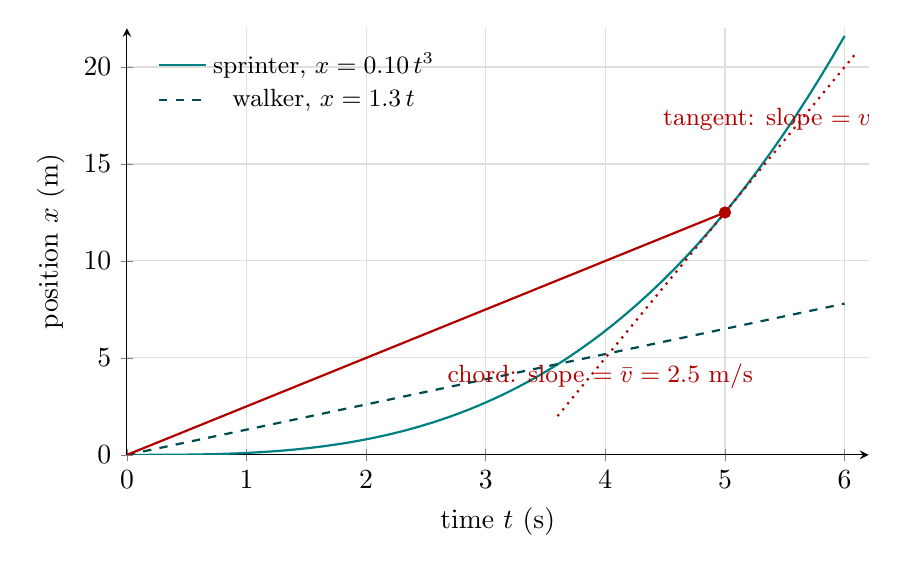
\begin{tikzpicture}
\begin{axis}[
  width=11cm,height=7cm,
  xlabel={time $t$ (s)},ylabel={position $x$ (m)},
  xmin=0,xmax=6.2,ymin=0,ymax=22,
  grid=major,grid style={gray!25},
  axis lines=left,
  legend pos=north west,legend style={font=\small,draw=none,fill=none},
]
\addplot[teal,thick,domain=0:6,samples=60] {0.10*x^3};
\addlegendentry{sprinter, $x = 0.10\,t^3$}
\addplot[teal!60!black,thick,dashed,domain=0:6,samples=2] {1.3*x};
\addlegendentry{walker, $x = 1.3\,t$}
% chord from 0 to 5
\draw[red!70!black,thick] (axis cs:0,0) -- (axis cs:5,12.5);
\node[red!70!black,font=\small,anchor=north west] at (axis cs:2.6,5.2) {chord: slope $= \bar v = 2.5$ m/s};
% tangent at t=5: slope 7.5, through (5,12.5)
\draw[red!70!black,thick,dotted] (axis cs:3.6,2.0) -- (axis cs:6.1,20.75);
\node[red!70!black,font=\small,anchor=west] at (axis cs:4.4,17.3) {tangent: slope $= v(5) = 7.5$ m/s};
\addplot[only marks,mark=*,mark size=2pt,red!70!black] coordinates {(5,12.5)};
\end{axis}
\end{tikzpicture}
\caption{Position--time graphs for the sprinter of Worked Example~\ref{ex:cubic} and for a walker at a steady \SI{1.3}{\metre\per\second}. A steady speed is a straight line whose slope is the speed. For the curved graph, the slope of the chord from $t = 0$ to $t = \SI{5}{\second}$ is the average speed over that interval, and the slope of the tangent at $t = \SI{5}{\second}$ is the instantaneous speed there.}
\label{fig:xt}
\end{figure}

\begin{twoviews}{slopes on a position--time graph}
\elem The walker's graph is a straight line. Between any two times the rise (distance covered) divided by the run (time elapsed) is the same, and it equals the speed; a straight position--time graph means steady speed, and a steeper line means a faster object. The sprinter's graph curves upward: it gets steeper, so the sprinter gets faster. The average speed over an interval is the slope of the \emph{chord} joining the two endpoints. The instantaneous speed at a moment is the slope of the line that just grazes the curve there, the \emph{tangent}, which you can estimate by laying a ruler along the curve.

\calc The slope of the chord from $t_1$ to $t_2$ is $[x(t_2) - x(t_1)]/(t_2 - t_1)$, the average speed. As $t_2 \to t_1$ the chord turns into the tangent, and its slope becomes $\dd x/\dd t$. That is the geometric meaning of the derivative, and Figure~\ref{fig:xt} is a picture of the limit in Definition~\ref{def:avginst}. Conversely, the area under a \emph{speed}--time graph is the distance covered, $\int v\,\dd t$. Slope takes you from position to speed; area takes you from speed back to position. Keep the pair in mind: Chapter~2 adds a third graph, of acceleration, to the stack.
\end{twoviews}

\begin{example}{The round-trip trap}{roundtrip}
You drive to a town \SI{60}{\kilo\metre} away at a steady \SI{60}{\kilo\metre\per\hour} and return along the same road at a steady \SI{40}{\kilo\metre\per\hour}. What is your average speed for the round trip? (It is not \SI{50}{\kilo\metre\per\hour}.)

\elem Average speed is total distance over total time, so find the total time. Outbound: $\SI{60}{\kilo\metre}/\SI{60}{\kilo\metre\per\hour} = \SI{1.0}{\hour}$. Return: $\SI{60}{\kilo\metre}/\SI{40}{\kilo\metre\per\hour} = \SI{1.5}{\hour}$. Total: \SI{120}{\kilo\metre} in \SI{2.5}{\hour}, so
\[
\bar v = \frac{\SI{120}{\kilo\metre}}{\SI{2.5}{\hour}} = \SI{48}{\kilo\metre\per\hour}.
\]
The average is below \num{50} because you spent \emph{more time} at the slower speed. Averaging speeds directly is only correct when the times spent at each speed are equal; here the distances were equal, which is different.

\calc The speed--time graph is two rectangles: height \num{60} for width \num{1.0}, then height \num{40} for width \num{1.5}. The mean value of $v$ is the total area over the total width:
\[
\bar v = \frac{\int_0^{2.5} v\,\dd t}{2.5} = \frac{60(1.0) + 40(1.5)}{2.5} = \frac{120}{2.5} = \SI{48}{\kilo\metre\per\hour}.
\]
The general result for equal distances $d$ at speeds $v_1$ and $v_2$ is $\bar v = 2d/(d/v_1 + d/v_2) = 2v_1 v_2/(v_1 + v_2)$, the \emph{harmonic mean}, which is always less than the ordinary mean unless $v_1 = v_2$ (Exercise~\ref{ex:harmonic}).\qed
\end{example}

\begin{checkbox}
A cheetah sprints \SI{100}{\metre} in \SI{4}{\second}. What is its average speed? Could it have reached that average without ever exceeding \SI{25}{\metre\per\second}? Could a car that starts from rest average \SI{80}{\kilo\metre\per\hour} over a trip without ever exceeding \SI{80}{\kilo\metre\per\hour}?
\end{checkbox}

\subsection{Speed relative to what?}

Every speed is measured relative to something. As you read this sentence, sitting still, you are moving at about \SI{30}{\kilo\metre\per\second} relative to the Sun as Earth swings around its orbit, and faster still relative to the centre of the galaxy. When we say a train moves at \SI{200}{\kilo\metre\per\hour}, we mean relative to the ground; a passenger walking toward the buffet car at \SI{1}{\metre\per\second} relative to the floor is moving at \SI{200}{\kilo\metre\per\hour} plus a little relative to the ground. Unless we say otherwise, speeds in this book are relative to the surface of Earth, which is what the tape measure and the stopwatch are attached to. The hunter's \SI{10}{\metre\per\second} means \SI{10}{\metre\per\second} relative to the mud.

\begin{checkbox}
A mosquito wants to hover directly above you as you rest in a hammock in a steady \SI{3}{\metre\per\second} breeze. How fast, and in what direction relative to the breeze, must it fly? (Adapted from Hewitt.)
\end{checkbox}
